\documentclass[a4paper,12pt,titlepage]{article}

\usepackage[german,ngerman]{babel}
\usepackage{fontspec}
\setmainfont{Calibri}
\usepackage{graphicx}
\usepackage{hyperref}
\usepackage{caption}

\begin{document}

\begin{titlepage}
    \centering
    \vspace*{2cm}
    {\LARGE\bfseries Automaten und formale Sprachen Blatt 4\par}
    \vspace{2cm}
    {\Large Jan Lucca Agricola (275867) \& Jakob Schulz (275258)\par}
    \vspace{2cm}
    {\large\today\par}
\end{titlepage}

\section{Aufgabe}
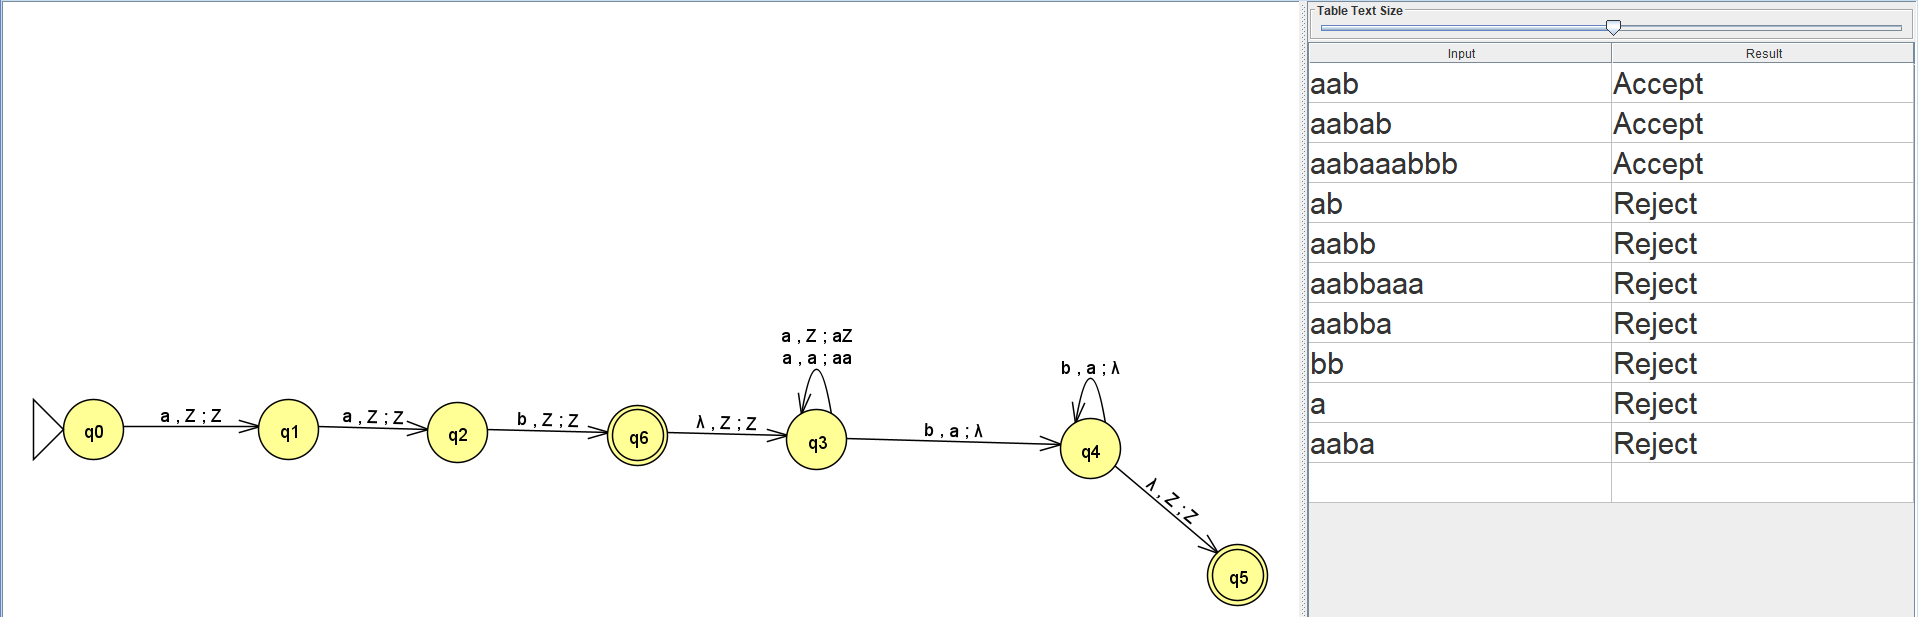
\includegraphics[width=1.0\textwidth]{task1.png}\\
\section{Aufgabe}
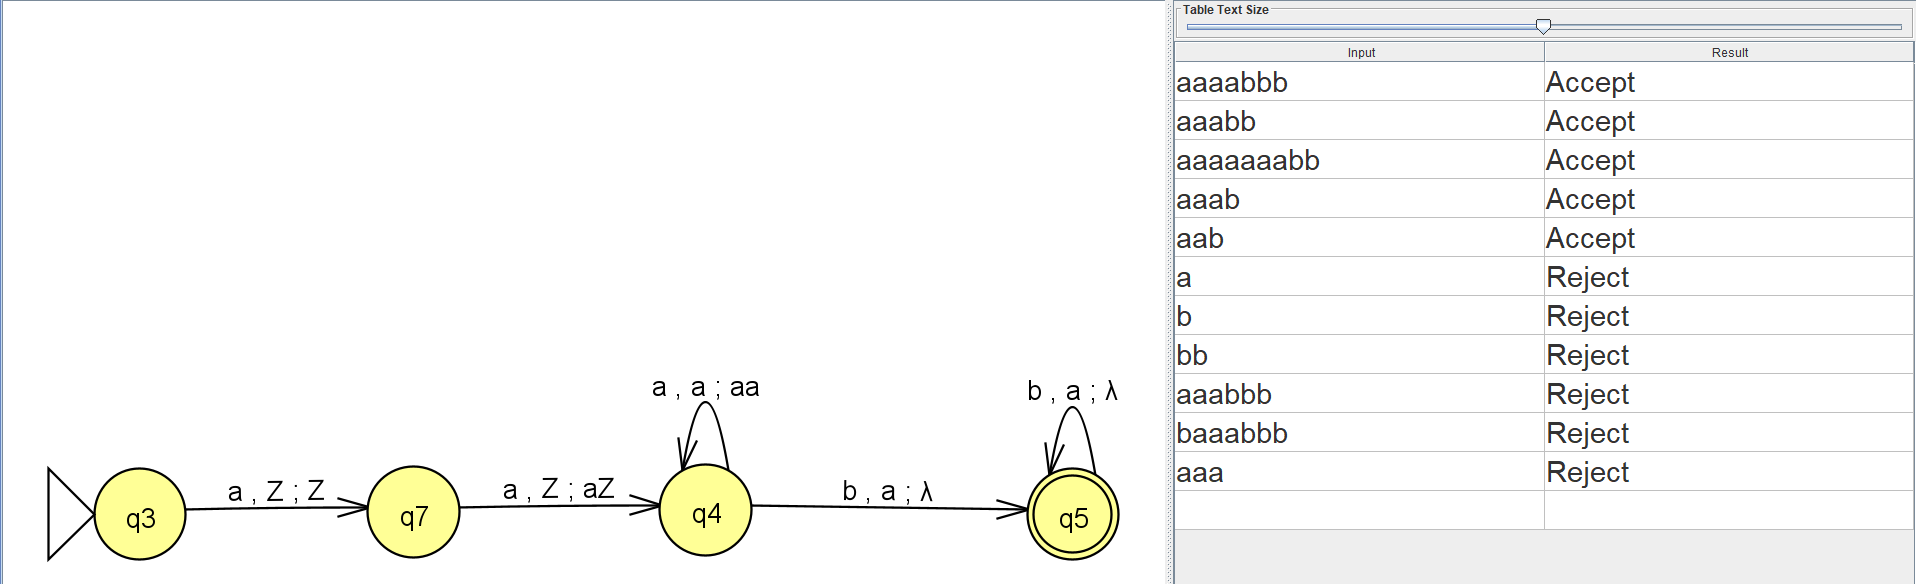
\includegraphics[width=1.0\textwidth]{task2.png}\\
\section{Aufgabe}
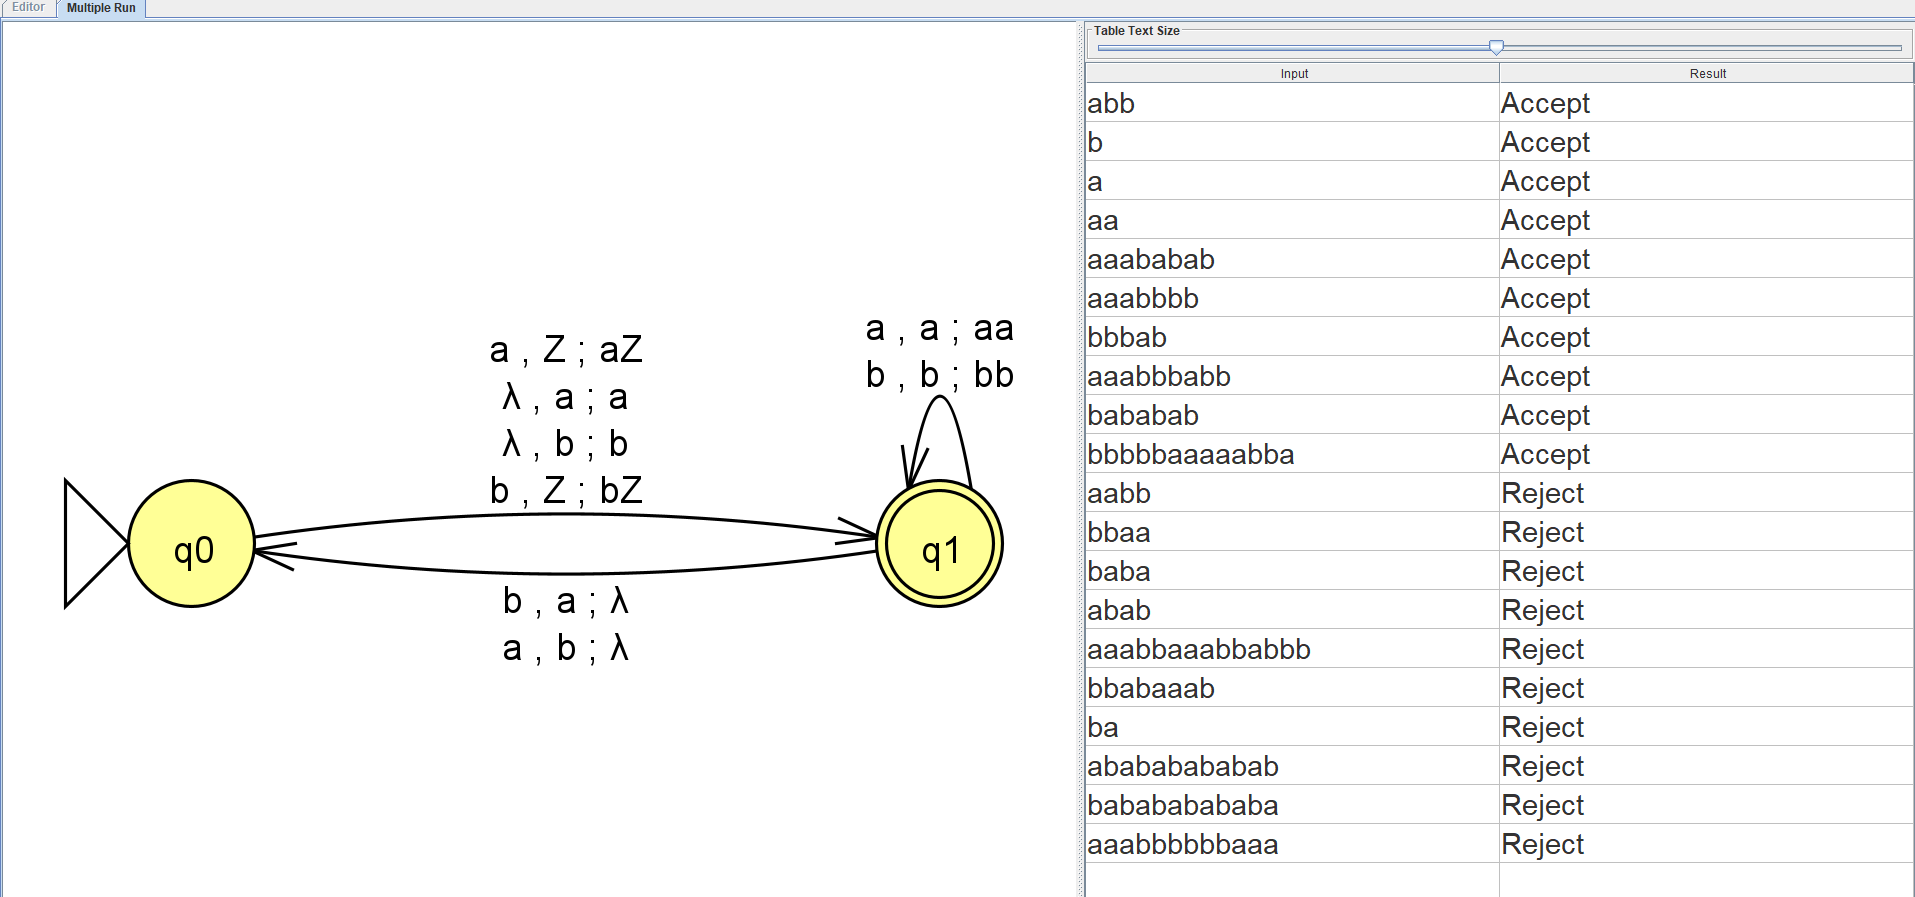
\includegraphics[width=1.0\textwidth]{task3.png}\\
\section{Aufgabe}
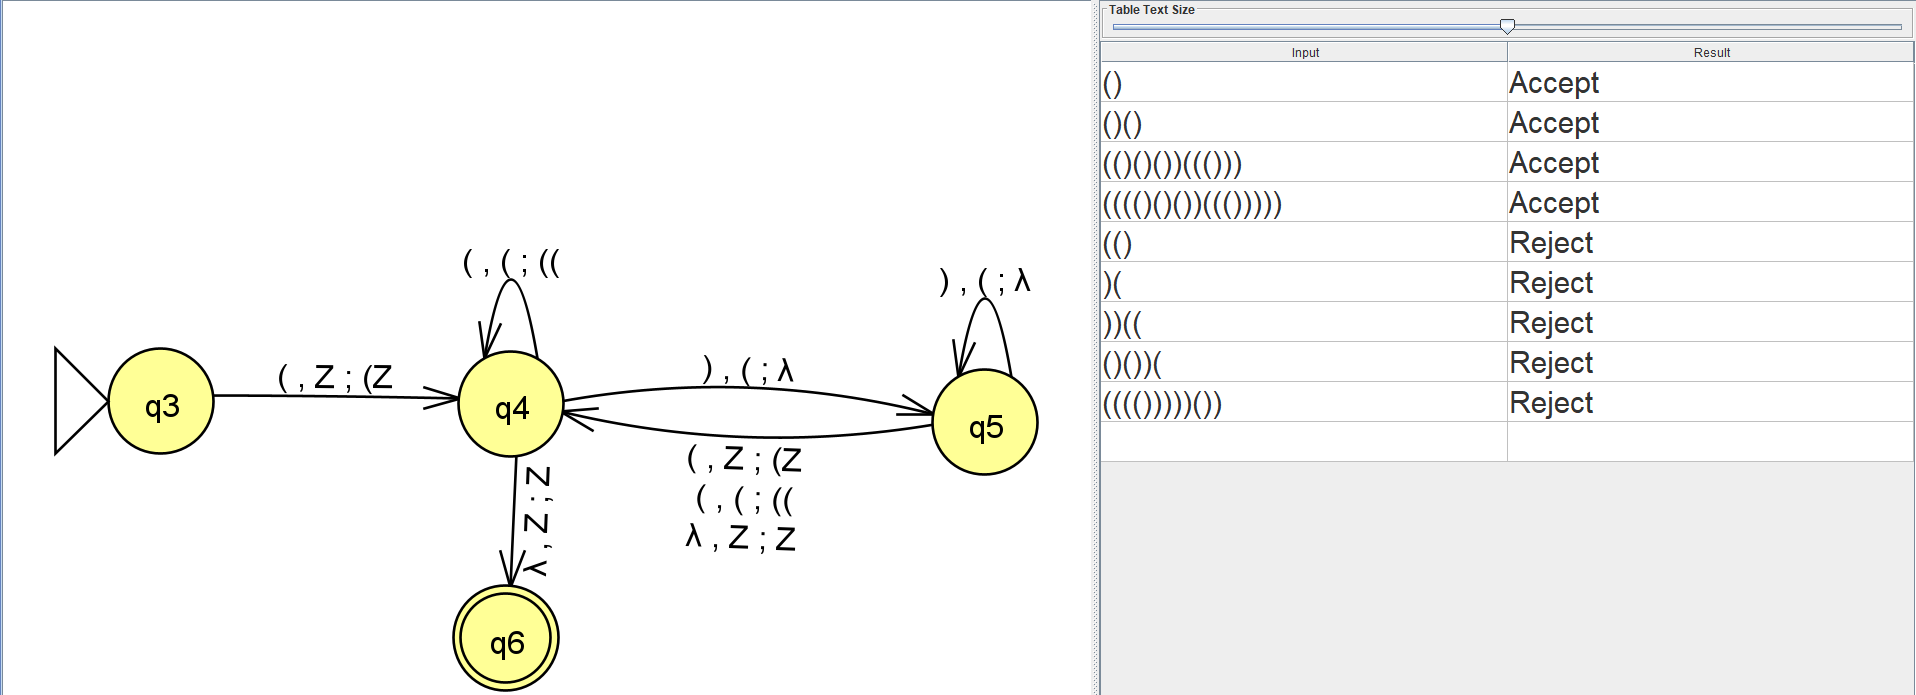
\includegraphics[width=1.0\textwidth]{task4.png}\\
\section{Aufgabe}
\subsection{Idee 1}
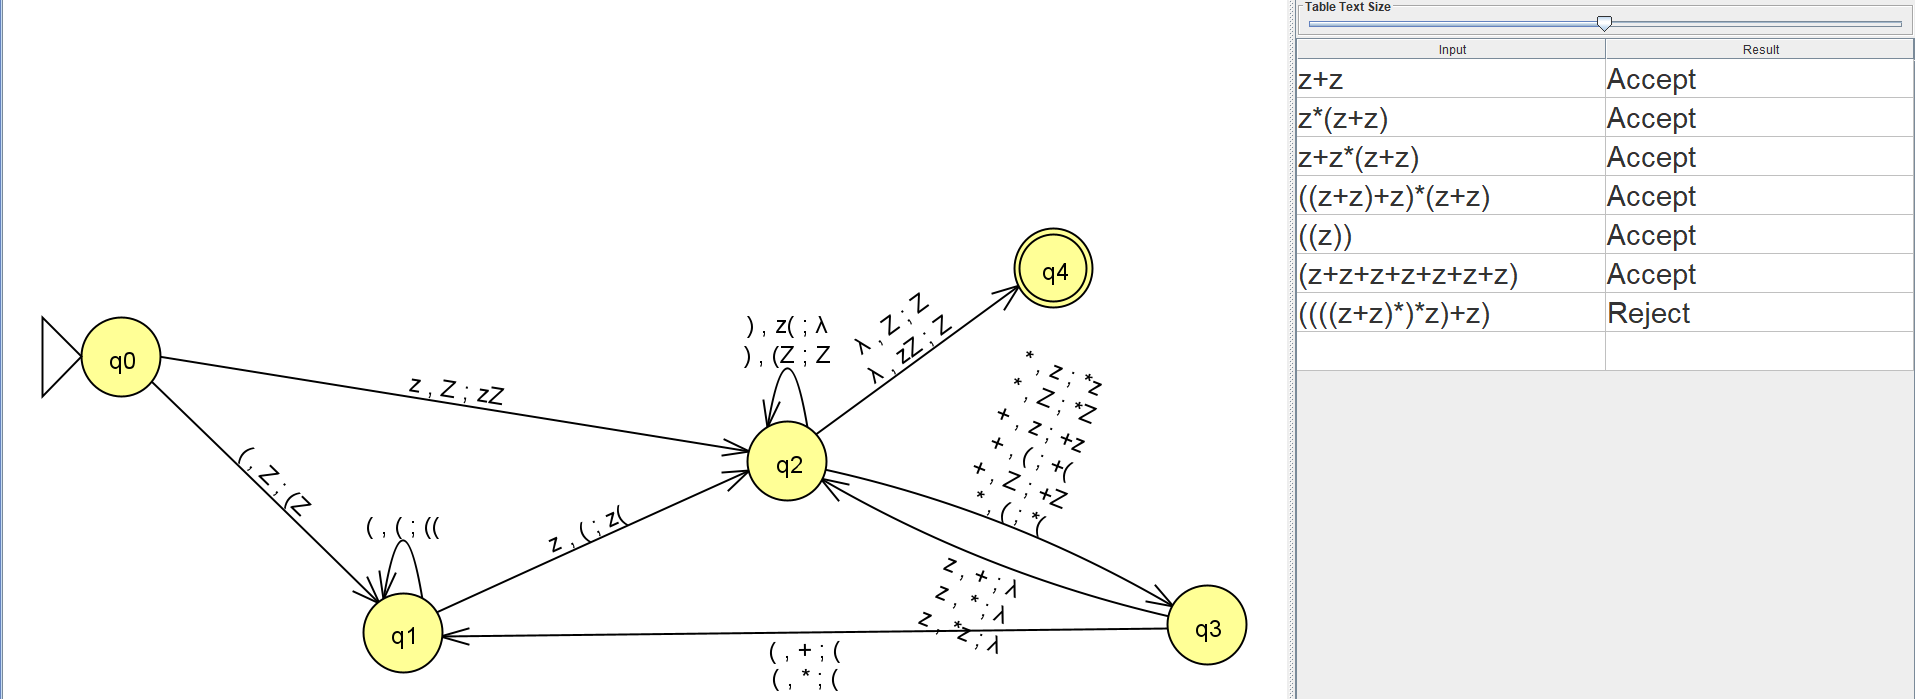
\includegraphics[width=1.0\textwidth]{task5SolutionJan.png}\\
\subsection{Idee 2}
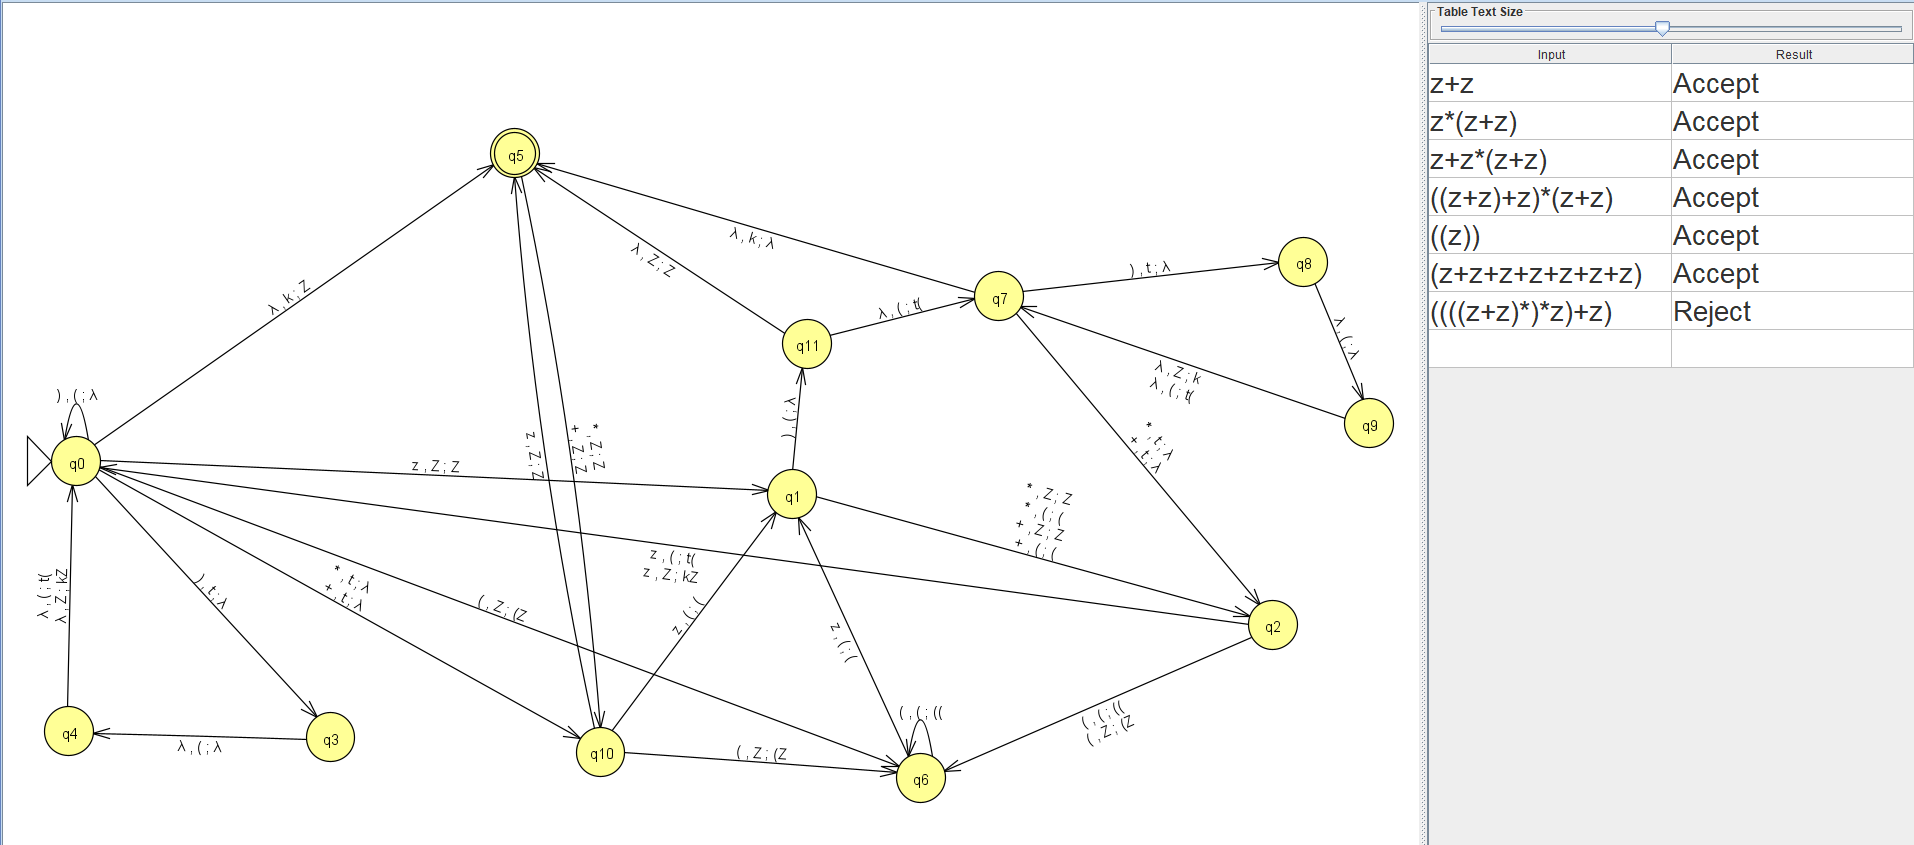
\includegraphics[width=1.0\textwidth]{task5SolutionJakob.png}\\
\begin{itemize}
\item k steht für \textbf{korrekter} Ausdruck
\item t steht für \textbf{teilweise korrekter} Ausdruck
\end{itemize}
\end{document}
